%==============================================================================
%  FINAL PROJECT PAPER  (IEEE Conference format)  --  Category A
%  GPU-accelerated vertical seam carving on a V100.
%
%  FIGURE ASSETS (Fig. 1): generated by cuda/seam_vis.cpp
%     figures/broadway_orig.jpg    original image
%     figures/broadway_seams.png   original with removed seams drawn red
%     figures/broadway_carved.png  image after removing the seams
%  Figs. 4-5 are HTML-generated, compiled to JPEG/PNG via rsvg-convert.
%  Fig. 6 (scaling) is a self-contained pgfplots.
%
%  METHOD NAMING (paper-facing):
%     Naive      = seam_carve_v0.cu   (one kernel launch per row)
%     Fused      = seam_carve.cu      (fused single-block, shmem ping-pong)
%     GridSync   = seam_carve_v3.cu   (multi-block grid.sync, abandoned)
%     Prefetch   = seam_carve_v4.cu   (+ software-pipelined energy prefetch)
%     BytePtr    = seam_carve_v5.cu   (+ 1-byte back-pointers)
%     Templated  = seam_carve_v6.cu   (+ compile-time width template; ≤4K)
%     GridStride = seam_carve_wide.cu (grid-stride, width-generic; runs 8K)
%     Tiled      = seam_carve_tiled_pf.cu (trapezoidal multi-SM + prefetch)
%
%  SECTION FILES:  paper/sections/sec_*.tex
%  TABLE FILES:    paper/tables/tab_*.tex
%==============================================================================
\documentclass[conference]{IEEEtran}
\IEEEoverridecommandlockouts

\usepackage{cite}
\usepackage{amsmath,amssymb,amsfonts}
\usepackage{newtxtext}
\usepackage{bm}
\usepackage{graphicx}
\usepackage{textcomp}
\usepackage{xcolor}
\usepackage{listings}
\usepackage{booktabs}
\usepackage{tikz}
\usetikzlibrary{positioning,arrows.meta,shapes.geometric,fit,matrix}
\usepackage{pgfplots}
\pgfplotsset{compat=1.16}
\usepackage{url}
\usepackage[hidelinks]{hyperref}

\newcommand{\mainbodyendpage}{?}
\AtEndDocument{%
  \typeout{====================================================}%
  \typeout{[PAGE BUDGET] Main body ends page \mainbodyendpage\space (limit: 6).}%
  \typeout{====================================================}%
}

\lstset{
  basicstyle=\ttfamily\footnotesize,
  breaklines=true, frame=single, columns=fullflexible,
  showstringspaces=false, keepspaces=true, xleftmargin=0.5em
}

\begin{document}

\title{How Far Can a GPU Push Exact Seam Carving? A Profiling-Driven Study of the Serial-Dependency Wall on a V100\\
{\footnotesize Final Project --- Parallel Programming, Spring 2026}}

\author{%
\IEEEauthorblockN{Yi-Wei Lien}
\IEEEauthorblockA{R14922062\\Dept.\ of CSIE\\National Taiwan University\\r14922062@ntu.edu.tw}
\and
\IEEEauthorblockN{Ya-Chen Wu}
\IEEEauthorblockA{R14944010\\Dept.\ of CSIE\\National Taiwan University\\r14944010@ntu.edu.tw}
\and
\IEEEauthorblockN{Yu-Hsiang Lo}
\IEEEauthorblockA{R14944037\\Dept.\ of CSIE\\National Taiwan University\\r14944037@ntu.edu.tw}%
}

\maketitle

%------------------------------------------------------------------------------
\begin{abstract}
Seam carving's dominant computation is a row-by-row dynamic program (DP) with
an irreducible top-to-bottom dependency. We ask how far a single GPU can push
\emph{exact} seam carving, and what fundamentally limits it. We build the
strongest exact pipeline we can on an NVIDIA V100 through a profiling-driven
optimization path---\textbf{\emph{Naive}}$\rightarrow$\textbf{\emph{Fused}}
(single-block shared-memory ping-pong)$\rightarrow$\textbf{\emph{Prefetch}}
(software-pipelined energy loads, the largest single win, after Nsight pins the
stall on global-load latency)$\rightarrow$\textbf{\emph{BytePtr}} (1-byte
back-pointers)$\rightarrow$\textbf{\emph{Tiled}}, a trapezoidal multi-SM kernel
that adapts shared-memory halo (ghost-cell) tiling to the DP with a seam-drift
correctness bound, activating all 80~SMs without per-row global synchronization.
\emph{Tiled} reaches \textbf{5.73\,ms/seam} at 8K ($7680{\times}4320$)---yet only
\textbf{6.2$\times$} over a tuned 32-thread NUMA-aware CPU baseline
($16$--$57\times$ over a single core, the metric prior GPU work reports).

This modest ceiling is \emph{structural}, and we establish it three ways. The
DP's critical path is provably irreducible---a transpose cannot reduce it---and,
unexpectedly, \emph{abandoning the DP altogether} for a greedy non-cumulative
selection gives no speedup either (${\approx}1.0\times$): the per-seam pipeline,
not the DP, is the end-to-end bottleneck. The only large lever is changing the
problem: an approximate batch mode that amortizes one pass over $K{=}60$ seams
reaches \textbf{56$\times$} over the exact pipeline (0.10\,ms/seam at 8K). Our
contribution is thus a characterization of \emph{why} exact seam carving resists
GPU acceleration, with the optimization study and impossibility arguments that
pin the achievable frontier. Output is bit-exact; a $3{\times}3$ sweep confirms
robustness.
\end{abstract}

\begin{IEEEkeywords}
seam carving, dynamic programming, CUDA, serial dependency, performance limits, V100
\end{IEEEkeywords}

\vspace{0.5em}
\noindent\fbox{\parbox{0.97\columnwidth}{\textbf{Project Category:}\quad
$\boxtimes$~\textbf{A} (Self-chosen topic)\qquad
$\square$~\textbf{B} (AI-agent code optimization)}}

%------------------------------------------------------------------------------
%------------------------------------------------------------------------------
\section{Introduction}
Digital image processing underpins virtually every modern visual application---from
content-delivery networks resizing thumbnails for billions of users to medical
imaging pipelines analysing high-resolution scans. On CPUs, pixel-count growth
translates directly into latency: operating on a $7680{\times}4320$ (8K) image
requires 33 million pixels per pass, each demanding arithmetic on every pipeline
stage. GPUs break this bottleneck for \emph{data-parallel} tasks.
Operations such as Gaussian blurring, histogram equalization, and convolution
map naturally to CUDA's SIMT model and routinely achieve orders-of-magnitude
acceleration over single-threaded CPU~\cite{cudaguide}.

Content-aware image resizing, however, breaks the data-parallel assumption.
Seam carving~\cite{avidan2007} preserves salient image content while changing
dimensions by iteratively removing \emph{seams}---connected pixel paths of
least visual importance. Its dominant computation is a row-by-row dynamic
program (DP, Eq.~\eqref{eq:dp}) with an
\textbf{irreducible serial chain} of $H$ dependent steps: each row's result
depends strictly on the row above it, and no reordering eliminates this
dependency. Figure~\ref{fig:carve} shows the visual effect;
Figure~\ref{fig:dpstages} illustrates the DP.

Prior GPU implementations have taken three approaches, each with a cost.
Duarte and Sendag~\cite{duarte2012} kept one kernel launch per DP row,
achieving 231$\times$ on the energy kernel but leaving the serial DP as the
system bottleneck. Kiess~et~al.~\cite{kiess2014} used global-atomic
busy-waits for row synchronization in one persistent kernel, reaching
10.5$\times$ at the cost of warp occupancy.
Kim~et~al.~\cite{kim2015} sidestepped the DP entirely with a
non-cumulative heuristic reaching 76.6$\times$---trading exactness for
throughput, a reasonable choice when batches of seams are removed at once; their
own \emph{exact} single-block DP reached only 5.9$\times$ and was abandoned.

This paper asks a deliberately two-sided question: \emph{how fast can the exact
seam-carve DP run on a single V100, and---more importantly---what fundamentally
limits it?} The answer turns out to be the interesting part: after exhausting the
optimization space we reach only $6.2\times$ over a strong CPU, and we show this
ceiling is \emph{structural}, not a failure of engineering effort. Our
contributions are therefore as much a \emph{characterization of the limit} as an
optimization study:
(i) the optimization itself---\textbf{\emph{Tiled}}, which adapts the ghost-cell
stencil pattern with a seam-drift correctness bound to run $K{\approx}60$ column
strips without per-row global synchronization (the supporting single-block path
\textbf{\emph{Fused}}$\rightarrow$\textbf{\emph{Prefetch}}$\rightarrow$\textbf{\emph{BytePtr}},
guided by Nsight, contributes $1.7$--$2.1\times$ from latency hiding alone);
(ii) two impossibility arguments---the DP critical path is irreducible and a
transpose cannot reduce it;
(iii) a falsified escape---abandoning the DP for a greedy non-cumulative
selection gives \emph{no} speedup (${\approx}1.0\times$, Appendix~\ref{app:greedy}),
showing the DP is not even the end-to-end bottleneck;
(iv) the one lever that works---an approximate batch mode (amortize one pass over
$K$ seams) reaching $56\times$. Together these pin where the achievable frontier
of exact seam carving on a GPU actually lies, and why.

\begin{figure}[t]
  \centering
  \newlength{\carvefigh}\setlength{\carvefigh}{2.0cm}
  \begin{minipage}[b]{0.32\columnwidth}\centering
    
\includegraphics[height=\carvefigh,width=\linewidth,keepaspectratio]{figures/broadway_orig.jpg}\\[1pt]
    {\scriptsize (a) Original}
  \end{minipage}\hfill
  \begin{minipage}[b]{0.32\columnwidth}\centering
    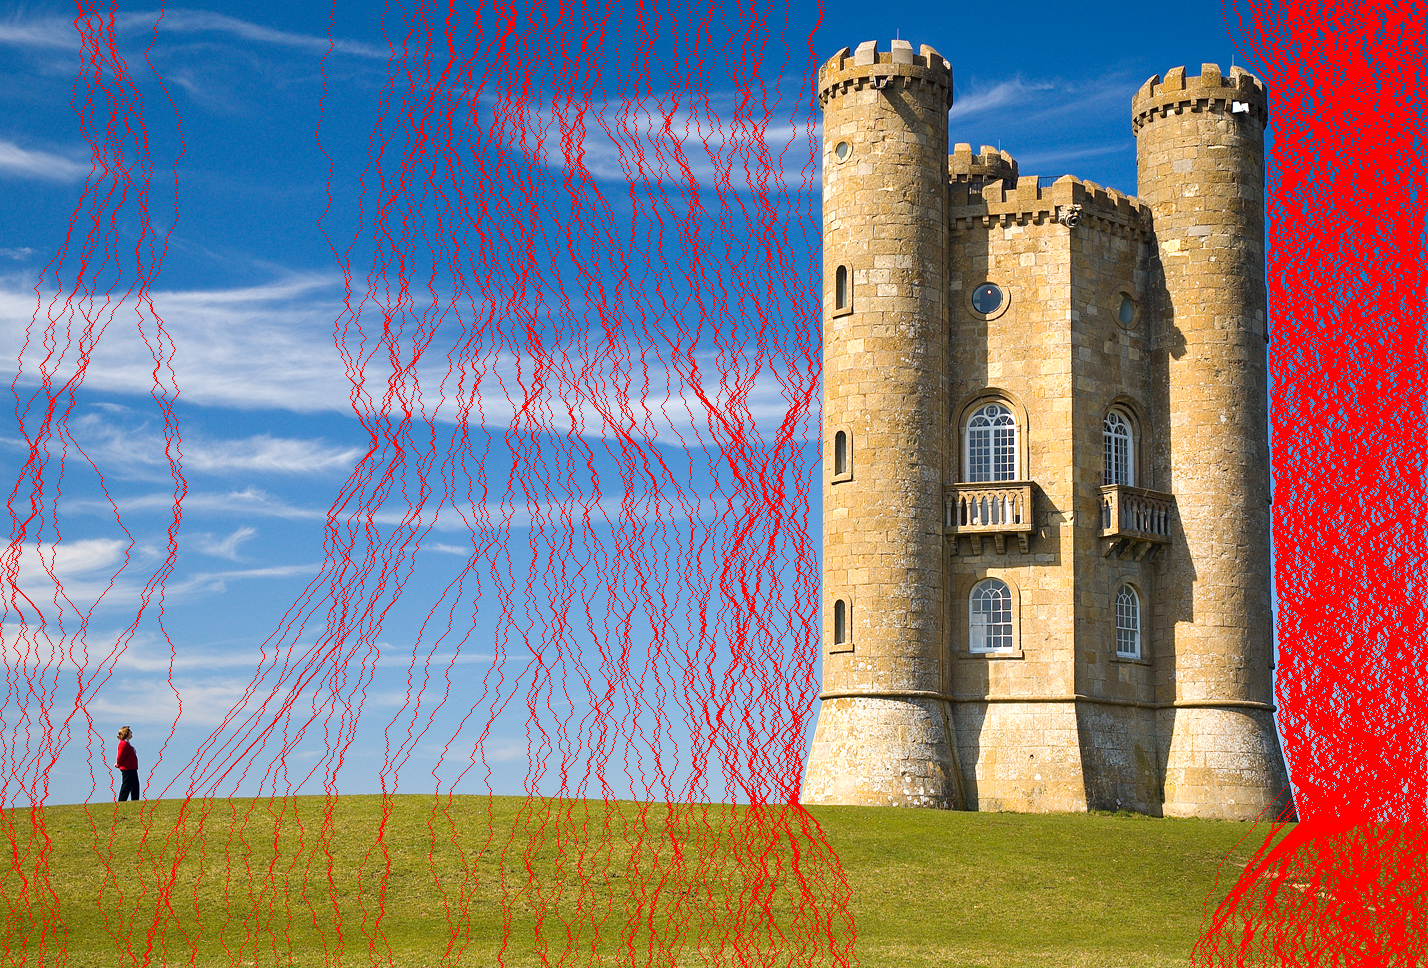
\includegraphics[height=\carvefigh,width=\linewidth,keepaspectratio]{figures/broadway_seams.png}\\[1pt]
    {\scriptsize (b) Seams (red)}
  \end{minipage}\hfill
  \begin{minipage}[b]{0.32\columnwidth}\centering
    
\includegraphics[height=\carvefigh,width=\linewidth,keepaspectratio]{figures/broadway_carved.png}\\[1pt]
    {\scriptsize (c) Carved}
  \end{minipage}
  \caption{Content-aware resizing: low-energy vertical seams (b) are removed
  iteratively, narrowing the image (c) while preserving salient structure.}
  \label{fig:carve}
\end{figure}


%------------------------------------------------------------------------------
%------------------------------------------------------------------------------
\section{Background and Related Work}

\textbf{Seam carving}~\cite{avidan2007} removes \emph{seams}---connected
pixel paths of least visual importance---to resize images in a
content-aware manner. For an image of size $H\!\times\!W$ with per-pixel energy
$e_{i,j}$ (gradient magnitude), the cumulative minimum-cost DP is
\begin{equation}
M_{i,j} = e_{i,j} + \min\!\bigl(M_{i-1,\,j-1},\;M_{i-1,\,j},\;M_{i-1,\,j+1}\bigr),
\label{eq:dp}
\end{equation}
with $M_{0,j}=e_{0,j}$. The optimal seam is recovered by back-tracking the
$\arg\min$ of the last row (Fig.~\ref{fig:dpstages}). Removing $k$ seams
repeats the full pipeline $k$ times. We resolve ties
left$\to$center$\to$right (strict ``$<$'') so all configurations are
bit-comparable.
Rubinstein~et~al.~\cite{rubinstein2008} extended the framework to video and
proposed \emph{forward energy}, which prefers seams that introduce less new
energy after removal, improving visual quality. Their formulation is a drop-in
replacement for our energy map and orthogonal to all GPU optimizations studied here.
Parallelizing the DP has been explored on CPUs: Stultz~\cite{stultz2008}
demonstrated an MPI decomposition but found Amdahl's law limits gains because
the row dependency serializes across partitions.
Lee and Kim~\cite{lee2009} proposed a \emph{partial-update} strategy---after
removing a seam, only the triangular influence region of the DP table is
recomputed---and a divide-and-conquer column decomposition; together these
halve per-seam DP work on CPU but require retaining the full $H{\times}W$
cost table in memory.
Mishiba and Ikehara~\cite{mishiba2011} partitioned the image into
blocks and computed seams independently per block, reducing recomputation
at the cost of seam continuity across boundaries---the CPU analogue of
\emph{Tiled}'s strip decomposition (Section~\ref{sec:method}).

Figure~\ref{fig:dpstages} illustrates the algorithm on a $4\times4$ toy image.

\begin{figure}[t]
\centering
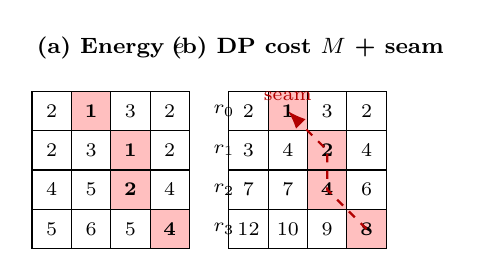
\begin{tikzpicture}[font=\scriptsize,
  cell/.style={draw,minimum size=5mm,inner sep=0pt},
  scell/.style={draw,minimum size=5mm,inner sep=0pt,fill=red!25,font=\bfseries\scriptsize}]

  % --- (a) Energy map ---
  \node[font=\footnotesize\bfseries] at (0.75,2.55) {(a) Energy $e$};
  \node[cell] at (0.0,1.75) {2}; \node[scell] at (0.5,1.75) {1};
    \node[cell] at (1.0,1.75) {3}; \node[cell] at (1.5,1.75) {2};
  \node[cell] at (0.0,1.25) {2}; \node[cell] at (0.5,1.25) {3};
    \node[scell] at (1.0,1.25) {1}; \node[cell] at (1.5,1.25) {2};
  \node[cell] at (0.0,0.75) {4}; \node[cell] at (0.5,0.75) {5};
    \node[scell] at (1.0,0.75) {2}; \node[cell] at (1.5,0.75) {4};
  \node[cell] at (0.0,0.25) {5}; \node[cell] at (0.5,0.25) {6};
    \node[cell] at (1.0,0.25) {5}; \node[scell] at (1.5,0.25) {4};

  % --- (b) DP cost table ---
  \node[font=\footnotesize\bfseries] at (3.25,2.55) {(b) DP cost $M$ + seam};
  % row 0
  \node[cell] at (2.5,1.75) {2}; \node[scell] at (3.0,1.75) {1};
    \node[cell] at (3.5,1.75) {3}; \node[cell] at (4.0,1.75) {2};
  % row 1
  \node[cell] at (2.5,1.25) {3}; \node[cell] at (3.0,1.25) {4};
    \node[scell] at (3.5,1.25) {2}; \node[cell] at (4.0,1.25) {4};
  % row 2
  \node[cell] at (2.5,0.75) {7}; \node[cell] at (3.0,0.75) {7};
    \node[scell] at (3.5,0.75) {4}; \node[cell] at (4.0,0.75) {6};
  % row 3 — argmin = col 3 (val 8)
  \node[cell] at (2.5,0.25) {12}; \node[cell] at (3.0,0.25) {10};
    \node[cell] at (3.5,0.25) {9}; \node[scell] at (4.0,0.25) {8};
  % row labels
  \node[left=0.5mm,font=\scriptsize] at (2.5,1.75) {$r_0$};
  \node[left=0.5mm,font=\scriptsize] at (2.5,1.25) {$r_1$};
  \node[left=0.5mm,font=\scriptsize] at (2.5,0.75) {$r_2$};
  \node[left=0.5mm,font=\scriptsize] at (2.5,0.25) {$r_3$};
  % back-track arrow
  \draw[-{Latex},red!70!black,thick,dashed]
    (4.0,0.25) -- (3.5,0.75) -- (3.5,1.25) -- (3.0,1.75)
    node[above,font=\scriptsize,red!70!black] {seam};
\end{tikzpicture}
\caption{Algorithm on a $4\times4$ toy image.
\textbf{(a)} Energy map $e_{i,j}$ (gradient magnitude); seam cells shaded.
\textbf{(b)} Cumulative DP cost $M_{i,j}$ (Eq.~\eqref{eq:dp}); the
minimum-cost path (shaded, dashed arrow) is back-tracked from
$\arg\min$ of $r_3$. Removing the shaded column yields a $4\times3$ image.}
\label{fig:dpstages}
\end{figure}

\textbf{GPU implementations of seam carving.}
Prior GPU work takes three distinct strategies. Duarte and
Sendag~\cite{duarte2012} kept the per-row-launch model (\emph{Naive} in our
terminology), achieving 231$\times$ on the energy kernel alone---but the DP
kernel, which launches one grid per row and reads/writes the full cost matrix
each time, remained the bottleneck.
Chiang~et~al.~\cite{chiang2009} used JND-based energy on GPU for real-time
video retargeting, exploiting data parallelism in the energy stage while
leaving the sequential DP row dependency unaddressed.
Kiess~et~al.~\cite{kiess2014} eliminated per-row launches for video retargeting
by spinning all threads in a single kernel with a global-atomic busy-wait for row
synchronization, reaching 10.5$\times$ on a GTX~650~Ti; the atomic spin wastes
warp slots and limits occupancy.
Kim~et~al.~\cite{kim2015} sidestepped the DP entirely with \emph{Non-Cumulative
Seam Carving} (NCSC), using raw per-pixel energy instead of cumulative
cost---a heuristic that gives 76.6$\times$ on a single GPU but sacrifices
exactness. Their own analysis (\S5.4) found that the exact single-block DP with
shared memory reached only 5.9$\times$ on their earlier-generation hardware,
which they deemed insufficient and abandoned. Without claiming hardware
equivalence, we revisit this \emph{design} and show profiling-driven latency
hiding makes the exact DP they discarded markedly more competitive. We do not
claim exactness is always preferable---where throughput dominates we approximate
too (batch mode, Section~\ref{sec:disc})---only that the choice deserves the
honest performance picture the abandoned exact DP lacked.

\textbf{CUDA optimization methodology.}
Harris~\cite{harris2007} characterized the performance of parallel reductions
on CUDA, establishing the principle of hiding global-memory latency with
arithmetic---the same technique our \emph{Prefetch} configuration applies to the
energy load in the DP inner loop. The V100's 80 SMs and 96\,KB per-block
shared-memory budget~\cite{voltawp} bound the design space of
Section~\ref{sec:method}.

\textbf{The multi-block barrier problem.}
Equation~\eqref{eq:dp}'s row dependency forces any naive multi-block DP to
synchronize across all SMs after every row (\textbf{$H$ global barriers per
seam}); we confirm this regresses $14\,\%$ behind \emph{Fused} on the V100
(\emph{GridSync}, Section~\ref{sec:results}).
Section~\ref{sec:method}'s \emph{Tiled} kernel resolves this with a halo
argument that reduces global syncs from $H$ to $H/T$, enabling $K{\approx}60$
active SMs without per-row coordination.


%------------------------------------------------------------------------------
%------------------------------------------------------------------------------
\section{Methodology}
\label{sec:method}

\textbf{Pipeline overview.}
The pipeline has four custom kernels: grayscale, energy, cost DP, and seam
removal (Fig.~\ref{fig:pipeline}).
Grayscale conversion uses BT.601 luma coefficients,
$Y = 0.299R + 0.587G + 0.114B$.
The energy map uses the $L_1$ gradient magnitude
\begin{equation}
e_{i,j} = \bigl|\partial I/\partial x\bigr| + \bigl|\partial I/\partial y\bigr|,
\end{equation}
computed with forward differences and border clamping.
The seam is extracted by back-tracking the \texttt{bp} array from
$j^{*} = \arg\min_{j}\,M_{H-1,j}$.
Profiling on a 1428$\times$968 image confirms the DP consumes $\bm{\sim}$\textbf{93\%}
of per-seam time; all optimization therefore targets that kernel.

\begin{figure}[t]
\centering
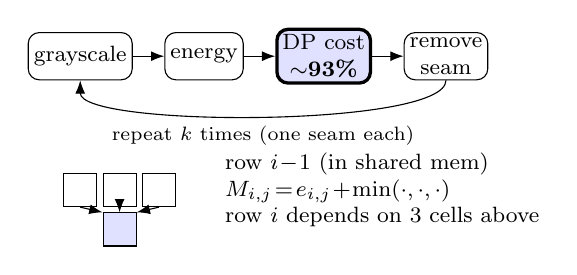
\begin{tikzpicture}[font=\footnotesize,node distance=3mm and 4mm]
  \tikzstyle{k}=[draw,rounded corners,minimum height=6mm,inner sep=2pt,align=center]
  \node[k] (g)  {grayscale};
  \node[k,right=of g] (e) {energy};
  \node[k,right=of e,fill=blue!12,very thick] (d) {DP cost\\\textbf{$\sim$93\%}};
  \node[k,right=of d] (r) {remove\\seam};
  \draw[-{Latex}] (g)--(e); \draw[-{Latex}] (e)--(d); \draw[-{Latex}] (d)--(r);
  \draw[-{Latex}] (r.south) .. controls +(0,-6mm) and +(0,-6mm) .. (g.south)
    node[midway,below,font=\scriptsize] {repeat $k$ times (one seam each)};
  \begin{scope}[shift={(0,-2.2)}]
    \foreach \x in {0,1,2} \node[draw,minimum size=4.2mm] (a\x) at (\x*0.5,0.5) {};
    \node[draw,minimum size=4.2mm,fill=blue!12] (b1) at (0.5,0) {};
    \draw[-{Latex}] (a0.south) -- (b1.north west);
    \draw[-{Latex}] (a1.south) -- (b1.north);
    \draw[-{Latex}] (a2.south) -- (b1.north east);
    \node[right=5mm of a2,align=left] {row $i\!-\!1$ (in shared mem)\\$M_{i,j}\!=\!e_{i,j}\!+\!\min(\cdot,\cdot,\cdot)$\\row $i$ depends on 3 cells above};
  \end{scope}
\end{tikzpicture}
\caption{The four-kernel pipeline (top) and the DP's 3-way row dependency
(bottom). The $H$ rows are serial; the $W$ columns within each row are parallel.}
\label{fig:pipeline}
\end{figure}

\begin{figure}[t]
\centering
\includegraphics[width=\columnwidth]{figures/fig_kerneldesign.jpeg}
\caption{Kernel paradigm comparison.
\textbf{Naive} launches $H$ kernels (one per row) with a global-memory
round-trip each time.
\textbf{Fused} collapses all rows into one kernel: rows exchange via a
shared-memory ping-pong with \texttt{\_\_syncthreads} between them.
\textbf{Tiled} runs $K$ blocks in parallel (one strip per SM); each tile of
$T$ rows stays entirely in shared memory and only exchanges one cost row
per strip through global memory at the tile boundary, reducing kernel
launches from $H$ to $\lceil H/T\rceil$.}
\label{fig:kerneldesign}
\end{figure}

\textbf{Naive} --- one kernel launch per row: $H{-}1$ launches per seam,
with a \textbf{full global-memory round-trip} per row
(Fig.~\ref{fig:kerneldesign}, left).
Each row reads $W$ energy and $W$ cost values from DRAM and writes $W$
cost values plus $W$ back-pointers back; total per-seam traffic is
$\bm{4HW}$ \textbf{memory transactions}, all of which hit DRAM because
the cost array (one seam at 4K: ${\sim}$32\,MB) far exceeds the L2 cache.

\textbf{Fused} --- one thread block walks all $H$ rows top-to-bottom, keeping
previous and current cost rows in two \textbf{ping-pong shared-memory buffers}
of $W$ \texttt{int16} values each (Fig.~\ref{fig:kerneldesign}, centre).
One \texttt{\_\_syncthreads()} separates rows, ensuring the prior row's
costs are visible before the next row begins.
Shared-memory footprint: $2W \times 2\,\text{B}$; at 4K ($W{=}3840$)
this is $15.4$\,KB, well within the 96\,KB opt-in limit.
One launch replaces $H$, eliminating $(H{-}1)$ kernel overheads.

\textbf{GridSync} --- replacing the block barrier with a grid-wide
\texttt{grid.sync()} after each row lets multiple SMs collaborate, but each of
the $H$ device-wide barriers costs ${\sim}10\,\mu\text{s}$ against only
${\sim}1\,\mu\text{s}$ of per-row arithmetic at $W{=}1428$: \textbf{barrier-bound
at $\bm{\sim}$6\% occupancy}, so we abandon it. This negative result motivates
\emph{Tiled}'s barrier-free design.

\textbf{Prefetch} --- Nsight Compute identifies \emph{Fused}'s dominant stall as
\texttt{long\_scoreboard}: every warp waits ${\sim}$200 cycles for the global
load of the current energy row $e_{i,\cdot}$.
The fix is software pipelining: while computing $M_{i,\cdot}$ (which only
reads shared-memory cost data), each thread \textbf{issues the global load
for $e_{i+1,\cdot}$} into a register array \texttt{e\_next[]}.
By the time \texttt{\_\_syncthreads()} completes and row $i{+}1$ begins,
the load has resolved---arithmetic and memory transfer overlap:
\begin{equation}
\underbrace{\text{compute}\;M_{i,\cdot}}_{\text{shmem reads}} \;\big\|\;
\underbrace{\text{load}\;e_{i+1,\cdot}}_{\text{global read}}.
\end{equation}

\textbf{BytePtr} --- the back-pointer at each cell is one of $\{-1,0,+1\}$,
yet \emph{Fused} stores it as a 4-byte \texttt{int}.
Switching to \texttt{signed char} (1\,byte) \textbf{cuts back-store traffic by
$\bm{4\times}$}: at 4K ($W{=}3840$, $H{=}2160$), the back-pointer array
shrinks from 32\,MB to 8\,MB per seam pass.
Output is bit-identical; the seam extraction reads the same values.

\textbf{Templated} --- the $W\le 2048$ cap in \emph{Prefetch}/\emph{BytePtr}
arises because the register array \texttt{e\_next[]} must have a fixed
compile-time size.
Making columns-per-thread (\texttt{CPT} $= \lceil W/\text{blockDim}\rceil$) a
\textbf{compile-time template parameter} lets the host select the right
instantiation at launch; all prefetch arrays remain register-resident.
At 4K: $\text{CPT}=4$, registers per thread ${\approx}24$.
At ${\ge}6$K: $\text{CPT}=8$, register count exceeds the per-block budget
and the compiler spills to local memory---\textbf{Templated fails at $\ge$6K}.

\textbf{GridStride} --- \emph{Templated}'s register overflow at 8K is caused by
the fixed-size prefetch arrays.
\emph{GridStride} replaces the CPT register array with a \textbf{scalar
prefetch variable}: each thread strides over columns $t,\;t{+}B,\;t{+}2B,\ldots$
(where $B{=}\text{blockDim.x}$), issuing one scalar prefetch load per stride.
Register count stays constant at any $W$, enabling \textbf{arbitrary-width support},
at the cost of losing the multi-element register-resident overlap that
\emph{Templated} achieves---hence \emph{GridStride} shows a
20--40\% latency deficit vs.\ \emph{Templated} on images where both run.

\textbf{Tiled} --- \emph{Templated} and \emph{GridStride} both use a
\emph{single block}, leaving 79 of 80 SMs idle.
\emph{Tiled} breaks this with a \textbf{halo argument}
(Figs.~\ref{fig:kerneldesign} right, \ref{fig:tiledhalo}): the $W$ columns
are divided into $K$ strips of center width $S = \lceil W/K \rceil$.
Strip $k$ covers columns $[kS - T,\;(k{+}1)S + T)$---i.e., $T$ halo columns on
each side---so $K$ blocks run concurrently, one per SM.

The correctness argument is a seam-drift bound: within a tile of $T$ rows, the
seam shifts by at most one column per row, so after $T$ rows it has drifted by
at most $T$ columns.
Any seam error is therefore contained within the $T$-column halo, and the
center $S$ columns are \textbf{bit-exact}.
Only the center strip of the cost row is written to the global ping-pong
buffer at each tile boundary; the halo is recomputed by the neighboring block
from its own center result.

Shared memory per block stores two ping-pong cost rows and one back-pointer row,
each of width $S{+}2T$:
\begin{equation}
\text{shmem} = 2(S{+}2T)\cdot 2\,\text{B}
             + (S{+}2T)\cdot 1\,\text{B}
             = 5(S{+}2T)\,\text{B}.
\label{eq:shmem}
\end{equation}
At $K{=}60$, $T{=}64$, $W{=}3840$: $S{=}64$ and
$\text{shmem} = 5{\times}192 = 960\,\text{B}$ per block---far below the
96\,KB limit.
\textbf{Kernel launches drop from $H$ to $\lceil H/T\rceil$}
(68 at 8K with $T{=}64$) while all $K{\approx}60$ SMs stay active.
Output is bit-exact against \emph{Templated}.
A 3$\times$3 parameter sweep ($K{\in}\{40,60,80\}$, $T{\in}\{32,64,128\}$)
shows all nine combinations land within ${\sim}5\%$ of the optimum
(Appendix~\ref{app:sweep}):
\textbf{the design is robust to parameter choice}.

\begin{figure}[t]
\centering
\includegraphics[width=\columnwidth]{figures/fig_tiledhalo.png}
\caption{\textbf{Tiled} strip and halo layout.
\textit{Top}: The $W$ columns are divided into $K$ strips; each strip is
extended by $T$ halo columns on each side (orange). Adjacent strips share
halo columns without a barrier.
\textit{Bottom}: Within a tile of $T$ rows, one block computes entirely in
shared memory. The seam drifts at most one column per row, so after $T$ rows
the error stays inside the orange halo; the blue center is bit-exact.
Only the center strip is written to \texttt{d\_next} at the tile boundary.}
\label{fig:tiledhalo}
\end{figure}


%------------------------------------------------------------------------------
%------------------------------------------------------------------------------
\section{Experimental Setup}
\label{sec:setup}
\textbf{Hardware.} NVIDIA V100 (\texttt{sm\_70}, 80 SMs, 96\,KB shared memory
opt-in) on the TWCC Taiwania-2 cluster, jobs placed by SLURM. The V100 is the
GPU class the course provides on this shared cluster---newer architectures are
not available to us---so we treat it as a fixed constraint; the techniques
studied (latency hiding, halo tiling, compact back-pointers) are
architecture-general, not Volta-specific. Nodes have 36 cores
and 8 GPUs; SLURM gates CPUs at ${\approx}4$ per GPU, so the multicore CPU
baseline reserves all 8 GPUs to obtain a 32-core allocation.

\textbf{Software.} CUDA 12.8, \texttt{nvcc -O3 -arch=sm\_70}; CPU code
\texttt{gcc -O3 -march=native -funroll-loops}. I/O via \texttt{stb\_image}.

\textbf{CPU baseline.} A host-side implementation mirrors the CUDA kernels
bit-for-bit (verified by \texttt{cmp} vs.\ the sequential reference). Our best
OpenMP variant keeps the team alive for the whole carve (one persistent parallel
region, not a per-row re-spawn), uses NUMA-aware parallel first-touch, and
ping-pongs the two live DP cost rows in cache. We report the CPU baseline as the
\emph{best ms/seam over 1--32 threads} (Appendix~\ref{app:omp}, optimum at
8--32); speedups are stated against both a single core and this configuration.

\textbf{Measurement.} We time the full carving loop (all four kernels, all
seams): \texttt{cudaEvent} on GPU, \texttt{std::chrono} on CPU.
We report \textbf{best-of-3} runs as \textbf{ms per seam} (50 seams unless
otherwise noted). Kernel-level profiling uses Nsight Compute (\texttt{ncu}).

\textbf{Workload.} Benchmarks use six resolutions spanning 0.52--33.2\,MP:
ctrl ($960{\times}540$), 1080p ($1920{\times}1080$), 2K ($2560{\times}1440$),
4K ($3840{\times}2160$), 6K ($6144{\times}3456$), 8K ($7680{\times}4320$).

\textbf{Correctness.} All configurations are compared with \texttt{cmp};
every configuration is bit-identical to every other on the resolutions it
supports. The deterministic tie-break guarantees a unique seam.


%------------------------------------------------------------------------------
%------------------------------------------------------------------------------
\section{Results}
\label{sec:results}
\textbf{Kernel-level progression.} Table~\ref{tab:versions} summarizes the DP
kernel on the 1428$\times$968 image (Nsight, first seam).
\textbf{\emph{Fused}} is the structural baseline; \textbf{\emph{GridSync}}
regresses (barrier-bound); \textbf{\emph{Prefetch}} removes the dominant
\texttt{long\_scoreboard} stall and gives the \textbf{largest single jump}
(\textbf{1.67$\times$}); \textbf{\emph{BytePtr}} trims store traffic to reach
the latency floor.

% Table I — DP kernel duration per configuration
% Protocol: Nsight Compute, first seam, 1428×968 (Broadway)
% Note: Prefetch and BytePtr speedups (1.67× and 1.85×) are consistent 
% across resolutions (1920×1080: 1.96× and 2.08×; 960×540: 1.95× and 1.97×).
\begin{table}[t]
\caption{DP kernel per configuration (1428$\times$968, Nsight, first seam).
\emph{Naive} uses $H$ per-row launches; no single fused kernel to profile.
Prefetch/BytePtr improvements verified consistent across standard resolutions.}
\label{tab:versions}
\centering
\begin{tabular}{@{}lcc@{}}
\toprule
\textbf{Method} & \textbf{Duration (ms)} & \textbf{vs \emph{Fused}} \\
\midrule
\emph{Naive}     & ---            & ---                        \\
\emph{Fused}     & 1.46           & 1.00$\times$ (baseline)    \\
\emph{GridSync}  & \textbf{1.66}  & \textbf{0.88$\times$} (regressed) \\
\emph{Prefetch}  & \textbf{0.872} & \textbf{1.67$\times$}      \\
\emph{BytePtr}   & 0.790          & 1.85$\times$               \\
\emph{Templated} & 0.790          & 1.85$\times$               \\
\bottomrule
\end{tabular}
\end{table}


\textbf{Hardware footprint (Table~\ref{tab:hw}).}
\emph{Fused} and \emph{GridStride} store the full $W$-wide cost row in
shared memory ($5W$ bytes), which reaches 37.5\,KB at 8K yet still fits
within the 96\,KB limit.
\emph{Tiled}'s per-block shared memory is fixed at 0.9\,KB regardless of
$W$ (from Eq.~\eqref{eq:shmem}), enabling 60 independent blocks to coexist
with negligible resource pressure.
Register counts decrease from \emph{Fused} (${\approx}$20) to \emph{Tiled}
(${\approx}$16): \emph{Tiled}'s per-strip loop has fewer live variables than
the CPT-unrolled single-block design.

% Table III — Kernel hardware footprint (transposed: methods as columns)
% Register counts from Nsight Compute; shmem calculated from kernel structure.
% Fused/GridStride shmem = 5W bytes (2×ping-pong int16 + back-ptr int8 per row).
% Tiled shmem = 5(S+2T) bytes from Eq.(3), constant regardless of W.
\begin{table}[t]
\caption{Kernel hardware footprint (register counts from Nsight Compute;
shared memory calculated from kernel structure).
\emph{Fused}/\emph{GridStride} shared memory scales with $W$;
\emph{Tiled}'s 0.9\,KB/block is independent of $W$ (Eq.~\eqref{eq:shmem}).}
\label{tab:hw}
\centering
\begin{tabular}{@{}lccc@{}}
\toprule
 & \emph{Fused} & \emph{GridStride} & \textbf{\emph{Tiled}} \\
 & (1428\,px) & (8K wide) & (8K wide) \\
\midrule
Reg / thread   & ${\approx}20$ & ${\approx}18$ & ${\approx}16$ \\
Shmem / block  & 7.0\,KB       & 37.5\,KB      & \textbf{0.9\,KB} \\
Active SMs     & 1             & 1             & \textbf{60} \\
\bottomrule
\end{tabular}
\end{table}


\textbf{End-to-end throughput.} Table~\ref{tab:fullresults} gives
whole-pipeline ms/seam for CPU (a single core and the best multicore OpenMP
configuration), \emph{Naive} GPU, the prior single-block best (\emph{Templated} at ${\le}4$K;
\emph{GridStride} at 6K--8K), and \emph{Tiled}.
All rows use the same 50-seam best-of-3 protocol.
Key observations:
\textbf{(1)} At ctrl--4K, \emph{Tiled} beats \emph{Templated} by
\textbf{$1.13$--$1.43\times$} while remaining bit-exact.
\textbf{(2)} At 6K/8K, \emph{Tiled} is \textbf{$2.6\times$} and
\textbf{$3.1\times$} faster than the prior best (\emph{GridStride}).
\textbf{(3)} Over the best multicore CPU baseline (NUMA-aware OpenMP, best of
1--32 threads; Appendix~\ref{app:omp}), \emph{Tiled}'s speedup grows
\emph{monotonically} from \textbf{3.6$\times$} (ctrl) to \textbf{6.2$\times$}
(8K)---larger images engage more of the 60\,SMs. Over a single CPU core the
range is \textbf{16$\times$}--\textbf{57$\times$}.
\textbf{(4)} Kim~et~al.~\cite{kim2015} found their \emph{exact} single-GPU DP
reached only $5.9{\times}$ on their earlier-generation hardware and abandoned
it for the approximate NCSC heuristic. Hardware differs, so this is a
\emph{design}-level point, not a normalized comparison: latency hiding makes
the exact DP they discarded scale well, removing the need to approximate.

% Table II — Full end-to-end ms/seam across all methods and resolutions
% Protocol: wall-clock, best-of-3, 50 seams
% † Templated fails at ≥6K (register overflow)
% ‡ CPU best: best ms/seam over 1–32 threads, NUMA-aware OpenMP (v4), see Appendix D
% Fused ctrl not benchmarked (single-block fits 540-row images but was not collected)
% GridStride: only benchmarked at 2K, 6K, 8K
\begin{table*}[t]
\caption{End-to-end ms/seam across all methods and resolutions (best-of-3, 50 seams).
\textbf{Bold} = best GPU result per resolution.
$\dagger$\emph{Templated} fails at ${\ge}6$K (register file overflow at CPT\,=\,8).
--- indicates not benchmarked or unsupported at that resolution.
$\ddagger$ \emph{CPU best} is the best ms/seam over 1--32 threads of our
NUMA-aware OpenMP baseline (persistent team, parallel first-touch, cache
ping-pong); the optimum lies at 8--32 threads (Appendix~\ref{app:omp}).}
\label{tab:fullresults}
\centering
\begin{tabular}{@{}lcccccc@{}}
\toprule
\textbf{Method} & \textbf{ctrl} & \textbf{1080p} & \textbf{2K} & \textbf{4K} & \textbf{6K} & \textbf{8K} \\
 & {\scriptsize 960$\times$540} & {\scriptsize 1920$\times$1080} & {\scriptsize 2560$\times$1440} & {\scriptsize 3840$\times$2160} & {\scriptsize 6144$\times$3456} & {\scriptsize 7680$\times$4320} \\
\midrule
CPU 1 core                   & 5.00  & 21.6  & 37.5  & 83.6  & 212   & 325   \\
CPU best$^\ddagger$          & 1.14  & 3.59  & 5.63  & 9.88  & 25.6  & 35.4  \\
\midrule
\emph{Naive}                 & 1.37  & 3.10  & 3.77  & 5.92  & 10.3  & 13.9  \\
\emph{Fused}                 & ---   & 1.94  & 3.08  & 6.73  & 12.63 & 21.3  \\
\emph{Templated}$\dagger$    & 0.355 & 1.08  & 1.57  & 3.10  & ---   & ---   \\
\emph{GridStride}            & ---   & ---   & 2.87  & ---   & 10.8  & 17.7  \\
\textbf{\emph{Tiled}} (ours) & \textbf{0.314} & \textbf{0.917} & \textbf{1.25} & \textbf{2.16} & \textbf{4.16} & \textbf{5.73} \\
\midrule
\emph{Speedup vs 1 core}     & 16$\times$ & 24$\times$ & 30$\times$ & 39$\times$ & 51$\times$ & \textbf{57$\times$} \\
\emph{Speedup vs CPU best}   & 3.6$\times$ & 3.9$\times$ & 4.5$\times$ & 4.6$\times$ & 6.2$\times$ & \textbf{6.2$\times$} \\
\bottomrule
\end{tabular}
\end{table*}


\textbf{Scaling in pixels (Fig.~\ref{fig:scaling}).}
\emph{Tiled}+Prefetch grows sublinearly: a 64$\times$ increase in pixels
(ctrl$\to$8K) costs only ${\sim}18\times$ more time
(0.314$\to$5.73\,ms/seam). Its slope is consistently below \emph{Templated}'s
on images where both run.

\begin{figure}[t]
\centering
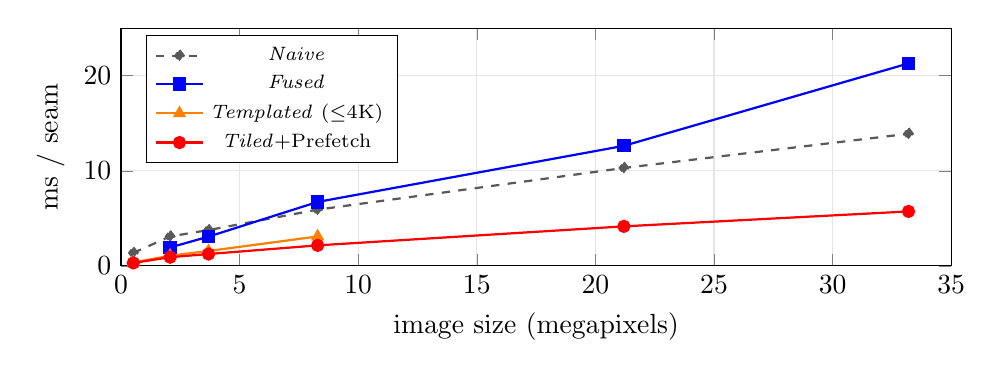
\begin{tikzpicture}
\begin{axis}[
  width=\columnwidth, height=4.6cm,
  xlabel={image size (megapixels)}, ylabel={ms / seam},
  xlabel near ticks, ylabel near ticks,
  xmin=0, xmax=35, ymin=0, ymax=25,
  legend pos=north west, legend style={font=\scriptsize},
  grid=major, grid style={gray!20},
  xtick={0,5,10,15,20,25,30,35},
]
% Naive: ctrl, 1080p, 2K, 4K, 6K, 8K (baseline: H launches, global R/W)
\addplot[mark=diamond*,gray!70!black,thick,dashed]
  coordinates {(0.52,1.37)(2.07,3.10)(3.69,3.77)(8.29,5.92)(21.2,10.3)(33.2,13.9)};
% Fused: 1080p, 2K, 4K, 6K, 8K (single-block, shared-mem ping-pong)
\addplot[mark=square*,blue,thick]
  coordinates {(2.07,1.94)(3.69,3.08)(8.29,6.73)(21.2,12.63)(33.2,21.3)};
% Templated: ctrl, 1080p, 2K, 4K (fails at 6K/8K, register overflow)
\addplot[mark=triangle*,orange,thick]
  coordinates {(0.52,0.355)(2.07,1.08)(3.69,1.57)(8.29,3.10)};
% Tiled+Prefetch: ctrl, 1080p, 2K, 4K, 6K, 8K
\addplot[mark=*,red,thick]
  coordinates {(0.52,0.314)(2.07,0.917)(3.69,1.25)(8.29,2.16)(21.2,4.16)(33.2,5.73)};
\legend{\emph{Naive}, \emph{Fused}, \emph{Templated} (${\le}4$K), \emph{Tiled}+Prefetch}
\end{axis}
\end{tikzpicture}
\caption{ms/seam vs.\ image size (0.52--33.2\,MP). \textbf{\emph{Tiled}+Prefetch}
has the lowest slope at all sizes and reaches \textbf{57$\times$} over CPU at 8K.
\emph{Templated} stops at 4K (register overflow). The gap to \emph{Fused}
widens with image size.}
\label{fig:scaling}
\end{figure}


%------------------------------------------------------------------------------
%------------------------------------------------------------------------------
\section{Discussion and Analysis}
\label{sec:disc}
\textbf{Why fusion is not free.} The most informative result is the 4K row of
Table~\ref{tab:fullresults}: \emph{Fused} (6.73\,ms) is barely faster than \emph{Naive}
(5.92\,ms) at 3840$\times$2160---a \textbf{$\sim$1.1$\times$} gain---whereas on small images
fusion gives \textbf{$1.6$--$1.7\times$}. Folding the whole DP into one block means one SM
chewing a 3840-wide row; its throughput cannot beat \emph{Naive}, whose per-row
launch spreads $W$ columns across all 80\,SMs. Fusion's benefit---eliminating $H$
launches---is large only when launch cost is a sizable fraction of per-row work,
which holds for narrow images but not for wide ones.
\textbf{Lesson: \emph{profile before assuming fusion wins}.}

\textbf{Latency hiding, not parallelism.} What improves the fused path at 4K is
latency hiding rather than added parallelism. \emph{Prefetch} overlaps the energy
load with arithmetic; \emph{BytePtr} quarters the back-store volume. Together
they take \emph{Templated} to $2.2\times$ over \emph{Naive} and $2.1\times$ over
\emph{Fused} at 4K, turning fusion's 4K break-even into a net gain.
Nsight Compute confirms: once \emph{BytePtr} is in place, \texttt{long\_scoreboard}
falls out of the top stall reasons entirely; the residual stalls are a balanced
mix of \texttt{not\_selected}, \texttt{wait}, and \texttt{barrier}---we have
reached the floor set by the serial row dependency.
By contrast, \emph{GridStride} (which cannot template-specialize its prefetch
arrays) shows \texttt{long\_scoreboard}$\approx$7 cycles as its top stall,
explaining its 20--40\,\% deficit vs.\ \emph{Templated} on images where both fit.

\textbf{Halo redundancy cost.}
\emph{Tiled} recomputes each strip's halo, so it performs more column work per
row than a single pass---a real arithmetic overhead, up to $3\times$ at 4K.
This is a deliberate trade-off: the alternative for exact multi-SM DP is a
device-wide barrier after every row, which we measured to be slower
(\emph{GridSync}). We quantify both sides below.
\emph{Tiled} computes $K{\times}(S{+}2T)$ columns per row instead of $W$,
where $S{=}W/K$ is the center-strip width. The \emph{redundancy factor} is
$\rho = 1 + 2TK/W$. At 4K ($W{=}3840$, $K{=}60$, $T{=}64$):
$\rho = 1 + 2{\times}64{\times}60/3840 = \mathbf{3.0{\times}}$.
At 8K ($W{=}7680$): $\rho = \mathbf{2.0{\times}}$.
Despite this overhead, the $K{=}60$ SM parallelism---unavailable to any
single-block design---dominates: an ideal linear model predicts
$60/\rho = \mathbf{20{\times}}$ throughput gain at 4K and $\mathbf{30{\times}}$ at 8K.
Measured gains over \emph{Fused} are \textbf{$3.1\times$} (4K) and \textbf{$3.7\times$} (8K),
reflecting that the V100's memory-bandwidth ceiling, not arithmetic capacity,
is the true limit. Halo overhead decreases as $W$ grows---\emph{Tiled}'s
efficiency therefore improves with resolution, matching the monotonically
widening speedup curve (Fig.~\ref{fig:scaling}).

\textbf{Limitations and multi-SM design.} (1) Single-block uses one SM, leaving
79/80 of the GPU idle during DP. \emph{Tiled} directly addresses this via the
halo argument: with $K{=}60$ strips and $T{=}64$ rows/tile, it achieves
\textbf{5.73\,ms/seam} at 8K (\textbf{$3.1\times$} over \emph{GridStride}). The
$3\times3$ parameter sweep confirms robustness: all combinations land within
${\sim}5\%$ of the optimum (Appendix~\ref{app:sweep}).
(2) \emph{Templated} fails at ${\ge}6$K: \texttt{CPT}=8 raises the per-thread
register count to ${\approx}$32, exhausting the V100's register file
at the required block size. We sidestep this with \emph{GridStride} (constant
registers via scalar prefetch) and \emph{Tiled} (${\approx}$16 registers/thread,
Table~\ref{tab:hw}), both register-safe at any width; rescuing \emph{Templated}
itself via explicit PTX-level register allocation is future work, as \emph{Tiled}
already supersedes it.
(3) The exact one-at-a-time formulation has been largely superseded in
production pipelines, which remove batches of seams in one forward pass at
the cost of pixel-exact reproducibility~\cite{kim2015}.
(4) Our NUMA-aware OpenMP baseline scales to 8--32 cores (Appendix~\ref{app:omp});
the optimum is limited by the per-row implicit barrier (small images) and
memory-bandwidth saturation (large images), not by thread-team management---the
team is persistent and pages are first-touched locally. \emph{Tiled} is
$3.6$--$6.2\times$ faster than this best multicore CPU configuration.
(5) Horizontal seams reuse the same kernels on a transposed image. We implement
a coalesced shared-memory transpose (Appendix~\ref{app:transpose}): it is
bit-exact, costs ${\approx}1.7$\,ms/pass at 8K, and adds only 0.14--0.25\%
when amortized over a multi-seam resize (though ${\approx}30\%$ for a single 8K
seam). The transpose only enables the orthogonal direction; it cannot
accelerate the DP itself, which we prove (critical-path invariance) and confirm
empirically in Appendix~\ref{app:depth}. The main results target vertical seams
to match prior GPU work.

\textbf{The DP is not the end-to-end bottleneck.}
At 8K the 5.73\,ms/seam splits into \textbf{${\approx}4.3$\,ms DP} (75\%) and
\textbf{${\approx}1.4$\,ms pre-processing} (25\%). Strikingly, \emph{removing}
the DP does not help---a greedy non-cumulative selection matches \emph{Tiled}
within 3\% (Appendix~\ref{app:greedy})---because every per-seam method pays the
same $\Omega(HW)$ memory-traffic floor (${\approx}1.4$\,ms) and the connected
seam search is $\Theta(HW)$-work either way; reducing the DP's depth below $H$
provably costs more work, not less (Appendix~\ref{app:greedy}). The only way
below the floor is to change the problem: \emph{read less} (incremental
update~\cite{lee2009}---bit-exact and $1.5\times$ on CPU, but no V100 win since
the tiled DP is latency-bound, Appendix~\ref{app:greedy}) or \emph{write less}
(batch, below)---the latter is our one large win.

\textbf{Extension to approximate multi-seam removal.}
The $K$-strip structure also supports batch removal: one DP pass yields $K{=}60$
strip-local seams that a single $K$-independent \emph{batch-remove} kernel
deletes in one pass, amortizing DP and preprocessing over 60 seams. We measured
(Appendix~\ref{app:batch}) \textbf{46$\times$} (ctrl) to \textbf{56$\times$} (8K)
over the exact single-seam pipeline---0.103\,ms/seam at 8K. This is the
practically important regime: the \emph{exact} pipeline leads the best multicore
CPU by only $6.2\times$ (serial-chain bound), whereas the approximate batch path
removes a seam every ${\approx}0.1$\,ms, two orders of magnitude below any
\emph{exact} CPU. The trade-off is strip-local, not global,
optimality~\cite{kim2015}; this mode is reported separately from the exact
contribution.

\textbf{No stronger exact CPU schedule.}
Diagonal-wavefront parallelization---which processes anti-diagonals $d{=}i{+}j$
for edit-distance-style DP---adds no parallelism here: cell $(i,j)$ depends on
$M_{i-1,j+1}$, whose anti-diagonal index is also $i{+}j{=}d$, so the dependency
lies within the same anti-diagonal. Row-parallel OpenMP ($W$-way per row, $H$
barriers) is therefore the natural exact CPU parallelization, and our baseline
is the best-tuned instance of it.

\textbf{Threats to validity.} Numbers are best-of-3 on a shared SLURM cluster;
we mitigate jitter by reporting ms/seam over 50 seams. The \emph{Naive} baseline
is a lean one-launch-per-row kernel; a less careful implementation would only
widen the gap, making our speedups over \emph{Naive} conservative.


%------------------------------------------------------------------------------
%------------------------------------------------------------------------------
\section{Conclusion}
We set out to find how fast exact seam carving can run on a V100, and the more
useful answer is \emph{where the wall is}. A profiling-driven path
(\emph{Fused}$\rightarrow$\emph{Prefetch}$\rightarrow$\emph{BytePtr}$\rightarrow$\emph{Tiled})
turns Nsight-diagnosed global-load latency into $1.7$--$2.1\times$ from latency
hiding, and \textbf{\emph{Tiled}}---a trapezoidal halo-tiled multi-SM DP---is the
best exact design at every resolution, reaching \textbf{5.73\,ms/seam} at 8K.
Yet that is only \textbf{6.2$\times$} over a tuned 32-thread CPU
($57\times$ over a single core). We show this ceiling is structural, not a lack
of effort: the DP critical path is irreducible, a transpose cannot reduce it,
and \emph{removing} the DP (greedy non-cumulative selection) gives no speedup
because the per-seam pipeline---not the DP---is the bottleneck. The one large
lever is amortization: approximate batch removal reaches $56\times$ over the
exact pipeline. The negative results (fusion's 4K break-even, \emph{GridSync}'s
barrier regression, the greedy wash) are as informative as the positive ones,
and a bit-exact shared-memory transpose adds horizontal seams for free
(Appendix~\ref{app:transpose}). Net: exact seam carving resists GPU acceleration
for structural reasons; meaningful speedup requires changing the problem, not
parallelizing harder.


%------------------------------------------------------------------------------
\begin{thebibliography}{00}
\bibitem{avidan2007} S.~Avidan and A.~Shamir, ``Seam carving for content-aware
image resizing,'' \emph{ACM Trans.\ Graphics}, vol.~26, no.~3, art.~10, 2007.
\bibitem{rubinstein2008} M.~Rubinstein, A.~Shamir, and S.~Avidan, ``Improved
seam carving for video retargeting,'' \emph{ACM Trans.\ Graphics}, vol.~27,
no.~3, art.~16, 2008.
\bibitem{stultz2008} J.~Stultz, ``Seam carving: Parallelizing a novel image
resizing algorithm,'' Tech.\ Rep., Brown Univ., 2008.
\bibitem{lee2009} J.~Lee and D.~Kim, ``Fast seam carving using partial update
and divide and conquer method,'' in \emph{Proc.\ Int.\ Symp.\ Signal Process.\
Inf.\ Technol.\ (ISSPIT)}, Ajman, UAE, pp.~107--112, Dec.~2009.
\bibitem{mishiba2011} K.~Mishiba and M.~Ikehara, ``Block-based seam carving,''
in \emph{Proc.\ Int.\ Symp.\ Access Spaces (ISAS)}, Yokohama,
pp.~111--115, Jun.~2011.
\bibitem{chiang2009} C.-H.~Chiang, S.-F.~Wang, Y.-L.~Chen, and S.-H.~Lai,
``Fast JND-based video carving with GPU acceleration for real-time video
retargeting,'' \emph{IEEE Trans.\ Circuits Syst.\ Video Technol.}, vol.~19,
no.~11, pp.~1588--1597, Nov.~2009.
\bibitem{kim2015} I.~Kim, J.~Zhai, Y.~Li, and W.~Chen, ``Optimizing seam
carving on multi-GPU systems for real-time image resizing,'' \emph{J.\
Supercomputing}, vol.~71, pp.~3500--3524, 2015.
\bibitem{kiess2014} J.~Kiess, D.~Gritzner, B.~Guthier, S.~Kopf, and
W.~Effelsberg, ``GPU video retargeting with parallelized SeamCrop,'' in
\emph{Proc.\ ACM Multimedia}, 2014.
\bibitem{duarte2012} R.~Duarte and R.~Sendag, ``Accelerating and characterizing
seam carving using a heterogeneous CPU-GPU system,'' in \emph{Proc.\ PDPTA},
2012.
\bibitem{harris2007} M.~Harris, ``Optimizing parallel reduction in CUDA,''
NVIDIA Developer Technology, Whitepaper, 2007.
\bibitem{voltawp} NVIDIA, ``NVIDIA Tesla V100 GPU Architecture,'' White Paper
WP-08608, 2017.
\bibitem{cudaguide} NVIDIA, ``CUDA C++ Programming Guide,'' v12.8, 2025.
\bibitem{nsight} NVIDIA, ``Nsight Compute Profiling Guide,'' 2025.
\bibitem{stb} S.~Barrett, ``stb\_image: public-domain image loader,''
\url{https://github.com/nothings/stb}.
\bibitem{maleki2014} S.~Maleki, M.~Musuvathi, and T.~Mytkowicz,
``Parallelizing dynamic programming through rank convergence,'' in
\emph{Proc.\ ACM PPoPP}, 2014, pp.~219--232.
\bibitem{jukna2015} S.~Jukna, ``Lower bounds for tropical circuits and dynamic
programs,'' \emph{Theory Comput.\ Syst.}, vol.~57, no.~1, pp.~160--194, 2015.
\end{thebibliography}

\xdef\mainbodyendpage{\thepage}

%==============================================================================
\appendices
\section{Crop-Ratio Sweep}
Table~\ref{tab:sweep} breaks down three methods across crop ratios
(5\%/10\%/20\%); ms/seam is nearly flat, confirming total time is linear in
seam count.

% Appendix Table — Full multi-resolution crop-ratio sweep
% Protocol: wall-clock, best-of-3, varying seam counts (5%/10%/20% of width)
% BytePtr limited to W≤2048 (fails at 3840-wide)
\begin{table}[h!]
\caption{ms/seam by image, crop ratio, and configuration (best-of-3).
ms/seam is nearly flat across crop ratios, confirming linear scaling in seam count.}
\label{tab:sweep}
\centering
\begin{tabular}{@{}llccc@{}}
\toprule
\textbf{Image} & \textbf{Crop} & \textbf{\emph{Fused}} & \textbf{\emph{BytePtr}} & \textbf{\emph{Templated}} \\
\midrule
Broadway          & 5\%  & 1.40 & 0.786 & 0.754 \\
1428$\times$968   & 10\% & 1.38 & 0.778 & 0.743 \\
                  & 20\% & 1.35 & 0.763 & 0.724 \\
\midrule
input1            & 5\%  & 1.73 & 1.02  & 0.958 \\
1920$\times$1080  & 10\% & 1.72 & 1.00  & 0.945 \\
                  & 20\% & 1.70 & 0.979 & 0.923 \\
\midrule
input             & 5\%  & 6.23 & ---   & 3.07  \\
3840$\times$2160  & 10\% & 6.20 & ---   & 3.02  \\
                  & 20\% & 6.22 & ---   & 2.94  \\
\bottomrule
\end{tabular}
\end{table}


\section{Batch Multi-Seam Results}
\label{app:batch}
Table~\ref{tab:batch} gives measured throughput for the approximate batch
multi-seam scheme described in Section~\ref{sec:disc}.
One DP pass produces $K{=}60$ seam candidates; a single batch-remove
kernel eliminates all $K$ in one image-wide read/write pass.

% Appendix Table — Batch multi-seam speedup
% Single: one seam per DP pass (exact, Tiled+Prefetch).
% Batch : K=60 seams per DP pass (approximate; batch-remove kernel).
% Speedup = single ms/seam ÷ batch ms/seam.
\begin{table}[h!]
\caption{Approximate batch multi-seam removal ($K{=}60$ seams per DP pass).
Single-seam baseline is \emph{Tiled}+Prefetch (exact).
Batch extracts $K$ strip-local seams from one DP pass and removes them
in a single GPU read/write pass over the image.}
\label{tab:batch}
\centering
\begin{tabular}{@{}lrrr@{}}
\toprule
\textbf{Resolution} & \textbf{Single (ms/seam)} & \textbf{Batch (ms/seam)} & \textbf{Speedup} \\
\midrule
ctrl  $960{\times}540$   & 0.279 & 0.0061 & $46{\times}$ \\
1080p $1920{\times}1080$ & 0.803 & 0.0162 & $50{\times}$ \\
2K    $2560{\times}1440$ & 1.226 & 0.0241 & $51{\times}$ \\
4K    $3840{\times}2160$ & 2.147 & 0.0401 & $54{\times}$ \\
6K    $6144{\times}3456$ & 4.147 & 0.0765 & $54{\times}$ \\
8K    $7680{\times}4320$ & 5.729 & 0.1028 & $56{\times}$ \\
\bottomrule
\end{tabular}
\end{table}


\section{Tiled \texorpdfstring{$K{\times}T$}{K×T} Parameter Sweep}
\label{app:sweep}
Table~\ref{tab:tilesweep} gives the full 3$\times$3 sweep results
supporting the robustness claim in Section~\ref{sec:method}.
The total spread across all nine $(K,T)$ combinations is
5.1\% at 4K and 4.1\% at 8K; the default $K{=}60$, $T{=}64$ lands within
1.2\% of the best configuration (1.2\% at 4K, 0.9\% at 8K).

% Appendix Table — Tiled K×T parameter sweep (ms/seam, with prefetch)
% Protocol: wall-clock, best-of-3, 50 seams.
% Data from results/tiled_sweep.md
% Bold = optimum per resolution. Default config: K=60, T=64.
\begin{table}[h!]
\caption{\emph{Tiled}+Prefetch ms/seam across the $3{\times}3$ parameter sweep
($K{\in}\{40,60,80\}$ strips, $T{\in}\{32,64,128\}$ rows/tile).
\textbf{Bold} = best per resolution; default ($K{=}60$, $T{=}64$) is within
1.2\% of the optimum at both resolutions.}
\label{tab:tilesweep}
\centering
\begin{tabular}{@{}cccc@{}}
\toprule
\multicolumn{4}{c}{\textbf{4K (3840$\times$2160) — ms/seam}} \\
\midrule
$K$ \textbackslash\ $T$ & $T{=}32$ & $T{=}64$ & $T{=}128$ \\
\midrule
$K{=}40$ & 2.247 & 2.169 & 2.146 \\
$K{=}60$ & 2.246 & 2.164 & 2.139 \\
$K{=}80$ & 2.245 & 2.165 & \textbf{2.139} \\
\midrule
\multicolumn{4}{c}{\textbf{8K (7680$\times$4320) — ms/seam}} \\
\midrule
$K$ \textbackslash\ $T$ & $T{=}32$ & $T{=}64$ & $T{=}128$ \\
\midrule
$K{=}40$ & 5.917 & 5.792 & 5.723 \\
$K{=}60$ & 5.901 & 5.738 & 5.696 \\
$K{=}80$ & 5.885 & 5.723 & \textbf{5.686} \\
\bottomrule
\end{tabular}
\end{table}


\section{CPU OpenMP Thread Scaling}
\label{app:omp}
Table~\ref{tab:omp} gives the full multicore scaling of our OpenMP baseline,
the source of the \emph{CPU best} row in Table~\ref{tab:fullresults}.
The implementation keeps the thread team alive for the entire carve (one
persistent parallel region, not a per-row re-spawn), first-touches every working
buffer in parallel so pages are NUMA-local to the socket that reads them, and
ping-pongs the two live DP cost rows in cache; it is bit-identical to the
sequential reference. Nodes are 36-core/8-GPU with SLURM gating ${\approx}4$
CPUs per GPU, so we reserve all 8 GPUs to obtain a 32-core allocation
(\texttt{OMP\_PROC\_BIND=close}, \texttt{OMP\_PLACES=cores}).
Scaling is strong to 8--32 threads; small images turn over near 8 (the per-row
barrier outweighs the shrinking per-row work) while large images keep improving
to 32 (bandwidth-bound). The previously reported regression past 4 threads was
an artifact of requesting only 4 CPUs and then oversubscribing them with up to
32 software threads---with a full allocation the curve is monotone to the
turn-over point.
(The OpenMP binary at one thread is ${\sim}15$--$20\%$ slower than the optimized
serial C++ reference used for the \emph{CPU 1 core} row of
Table~\ref{tab:fullresults}, hence the two tables' single-thread entries differ;
the multicore optimum, identical in source, is what the speedups use.)

% Appendix Table — TRUE multicore OpenMP thread-scaling (best-of-3, ms/seam).
% Binary: seam_carve_omp_v4 (persistent parallel region + NUMA-aware parallel
% first-touch + 2-row cache ping-pong), gcc -O3 -march=native -funroll-loops.
% Allocation: 8 GPUs reserved on a 36-core/8-GPU node to obtain 32 host cores
% (SLURM gates ~4 CPUs per GPU). OMP_PROC_BIND=close, OMP_PLACES=cores.
% Source: bench/sbatch_omp_final.sh, results/omp_scaling_full.md.
\begin{table}[h!]
\caption{True multicore OpenMP thread-scaling (ms/seam, best-of-3) of our
NUMA-aware baseline. \textbf{Bold} = best per resolution. The optimum is at
8--32 threads; small images turn over earlier (per-row barrier cost), large
images keep scaling (bandwidth-bound). The earlier ``regression past 4 threads''
was an artifact of a 4-CPU job allocation oversubscribed by higher thread
counts, not the algorithm.}
\label{tab:omp}
\centering
\begin{tabular}{@{}lrrrr@{}}
\toprule
\textbf{Threads} & \textbf{ctrl} & \textbf{1080p} & \textbf{4K} & \textbf{8K} \\
\midrule
1  & 5.58 & 25.03 & 101.13 & 394.37 \\
2  & 3.01 & 13.05 & 51.76  & 197.93 \\
4  & 1.71 & 7.05  & 27.21  & 103.73 \\
8  & \textbf{1.14} & 4.13 & 15.01 & 55.55 \\
16 & 1.34 & \textbf{3.59} & 10.45 & 37.55 \\
24 & 2.66 & 5.24 & 10.13 & 35.79 \\
32 & 3.54 & 6.50 & \textbf{9.88} & \textbf{35.42} \\
\bottomrule
\end{tabular}
\end{table}


\section{Horizontal Seams via VRAM Transpose}
\label{app:transpose}
Horizontal seam carving reuses the entire vertical pipeline unchanged: we
transpose the image once with a coalesced shared-memory kernel
(32$\times$32 tiles, padded to avoid bank conflicts), remove all $N$ seams in
the transposed orientation, then transpose back. The transpose is therefore a
fixed two-pass cost, not a per-seam one.
Table~\ref{tab:transpose} reports measured numbers. The transpose is bit-exact
(a round-trip reproduces the input with zero mismatches over 24.9\,M values at
4K) and the horizontal output is pixel-identical to an independent
transpose-carve-transpose reference.
Each transpose moves the whole image twice (read+write); at 8K this is
${\approx}1.7$\,ms/pass, ${\approx}3.4$\,ms for the round trip.
Amortized over a multi-seam resize the overhead is \textbf{0.14--0.25\%}
(Table~\ref{tab:transpose}); for a \emph{single} horizontal seam at 8K, however,
the 3.4\,ms transpose is ${\approx}30\%$ of the 8.0\,ms cost---the one case
where the transpose is not hidden.
Note that carving is slower per seam in the transposed orientation
(7.97 vs 5.73\,ms/seam at 8K): the DP serial chain then spans the original
\emph{width} (7680 rows) rather than the height (4320), an algorithmic
asymmetry independent of the transpose itself.

% Appendix Table — VRAM transpose cost and horizontal-carve breakdown.
% Protocol: V100, best-of-3, CUDA events. Source: bench/sbatch_transpose.sh.
% Transpose verified bit-exact (round-trip) and h-mode pixel-identical to an
% independent PIL-transpose -> vertical-carve -> PIL-transpose path.
\begin{table}[h!]
\caption{VRAM transpose cost and horizontal seam-carving breakdown (V100,
best-of-3). The transpose is a fixed two-pass overhead amortized over all $N$
removals. ``Carve'' is per-seam DP time in the transposed orientation, where the
serial chain length equals the original \emph{width}.}
\label{tab:transpose}
\centering
\begin{tabular}{@{}lrrrr@{}}
\toprule
\textbf{Resolution} & \textbf{Transp.\ in} & \textbf{Transp.\ out} &
\textbf{Carve} & \textbf{Overhead} \\
 & (ms) & (ms) & (ms/seam) & (\%, $N$) \\
\midrule
ctrl 960$\times$540   & 0.08 & 0.02 & 0.424 & 0.25\,(96)  \\
4K 3840$\times$2160   & 0.52 & 0.36 & 3.22  & 0.14\,(200) \\
8K 7680$\times$4320   & 1.81 & 1.63 & 7.97  & 0.22\,(200) \\
\bottomrule
\end{tabular}
\end{table}


\section{Why Transpose Cannot Accelerate the DP}
\label{app:depth}
A natural question is whether the transpose of Appendix~\ref{app:transpose}
could \emph{accelerate} seam carving rather than merely enable horizontal seams.
It cannot, for two reasons.

\textbf{(1) The critical path is transpose-invariant.}
Equation~\eqref{eq:dp} defines a dependency DAG in which node $(i,j)$ has
in-edges from $(i{-}1,j{-}1)$, $(i{-}1,j)$, $(i{-}1,j{+}1)$. Its longest
directed path has length $H$ (one node per row), so any schedule needs at least
$H$ sequential \texttt{min} steps. A transpose is a bijection $\sigma(i,j){=}(j,i)$
on storage addresses; relabeling storage leaves the dependency graph---and hence
its critical path---unchanged. Applying the DP to the transposed image instead
computes the \emph{orthogonal} (horizontal) seams, whose critical path is $W$.
Thus transpose either keeps the task and its depth $H$, or switches to the
orthogonal task with depth $W$; in neither case is the depth of a \emph{given}
task reduced.

\textbf{(2) The DP is already coalesced.}
In the column-parallel schedule, threads indexed by $j$ read the contiguous,
unit-stride addresses $M_{i-1,j-1}, M_{i-1,j}, M_{i-1,j+1}$ and $e_{i,j}$, so global transactions
are already fully coalesced. Transpose maps unit-stride-in-$j$ to
unit-stride-in-$i$, a symmetric change with no reduction in transactions.
Transpose is the standard remedy for \emph{uncoalesced} access; here there is
nothing to remedy.

\textbf{Consequence.}
Per-seam latency follows $T \approx D\cdot\tau(P)$, with serial depth $D$ and a
per-step time $\tau(P)$ that is non-increasing in the parallel width $P$.
Transpose maps $(D,P){\to}(P,D)$ but never lowers $D$ for a fixed seam
direction, so it can only add cost. The same holds for batch carving, whose
dominant term is the identical depth-$D$ DP (Appendix~\ref{app:batch}).
Table~\ref{tab:depth} confirms this directly: carving one image in both
orientations (identical $H{\cdot}W$ work, only $D$ changed), the larger-$D$
orientation is always slower---for both single-seam and batch---by a factor that
grows with $D$ (sublinearly, since larger $D$ pairs with larger $P$).
Transpose's only role is therefore enabling the orthogonal seam direction
(Appendix~\ref{app:transpose}); it offers no route to a faster DP.

% Appendix Table — depth-invariance controlled experiment.
% Same image, two orientations: identical H*W work, only serial depth D differs.
% Source: bench/sbatch_depth_invariance.sh (V100, best-of-3).
\begin{table}[h!]
\caption{Transpose changes orientation, not cost. The same image is carved in
both orientations: total work $H{\cdot}W$ is identical; only the DP serial depth
$D$ differs. The larger-$D$ orientation is \emph{always} slower---for both
single-seam and batch---confirming that performance tracks serial depth, which
transpose cannot reduce for a fixed seam direction.}
\label{tab:depth}
\centering
\begin{tabular}{@{}llrrr@{}}
\toprule
\textbf{Image} & \textbf{Orient.} & \textbf{Depth $D$} &
\textbf{Single} & \textbf{Batch} \\
 & & (rows) & (ms/seam) & (ms/seam) \\
\midrule
4K & original   & 2160 & \textbf{2.156} & \textbf{0.048} \\
4K & transposed & 3840 & 3.235 & 0.069 \\
\midrule
8K & original   & 4320 & \textbf{5.747} & \textbf{0.122} \\
8K & transposed & 7680 & 7.999 & 0.147 \\
\bottomrule
\end{tabular}
\end{table}


\section{A Per-Seam Lower Bound: Why Non-DP Cannot Win}
\label{app:greedy}
The question is not merely whether our greedy attempt happened to fail, but
whether \emph{any} selection---DP or not---can be faster on the V100. We argue it
cannot, via a method-independent lower bound, and confirm it empirically.

\textbf{(1) Bandwidth floor (method-independent).}
Removing one \emph{content-aware} seam must read every pixel's energy at least
once---otherwise an adversary places the minimum seam through an unread
pixel---and must write the $H{\times}(W{-}1)$ output; both are $\Omega(HW)$ words.
At 8K the image (398\,MB) far exceeds the V100's 6\,MB L2, so this traffic hits
DRAM. With peak bandwidth $\beta{\approx}900$\,GB/s,
$T_\text{seam} \ge 2\,(\text{image bytes})/\beta \approx 1.4$\,ms,
\emph{independent of how the seam is selected}. This matches our measured
pre-processing floor and the published estimate that energy recomputation alone
is ${\approx}25\%$ of seam-carving bandwidth~\cite{kim2015}. Exact DP, greedy,
and NCSC all pay it.

\textbf{(2) The DP is work-optimal.}
Finding the minimum-cost connected seam must inspect each of the $HW$ energies,
so $\Omega(HW)$ work is necessary; the cumulative DP does $\Theta(HW)$. Greedy
multi-start also does $\Theta(HW)$, but with column-scattered, cache-missing
access---which is exactly why it is no faster (Table~\ref{tab:greedy}).

\textbf{(3) Reducing depth costs work.}
The DP is a scan over associative $(\min,+)$ (tropical) transfer matrices, so by
associativity it parallelizes to $O(\log H)$ depth~\cite{maleki2014}. But the
banded transfers widen under composition, making the scan cost
$\Theta(HW\!\cdot\!\min(H,W))$ work---a factor ${\approx}4320$ above the serial
DP at 8K (${\sim}10^{11}$ tropical ops, tens of ms), \emph{strictly slower}.
Tropical-circuit lower bounds~\cite{jukna2015} indicate this blow-up is intrinsic.
Sub-$H$ depth is therefore counterproductive: the serial-depth, work-optimal DP
is the right operating point, not a deficiency.

\textbf{(4) We are near the frontier.}
Combining (1)--(3), per-seam time is bounded below by a $\Theta(HW)$-work
selection plus $\Omega(HW)$ traffic; \emph{Tiled}'s 5.73\,ms at 8K is within
${\approx}1.3\times$ of this floor (${\approx}4.3$\,ms selection $+$
${\approx}1.4$\,ms traffic). Little exact headroom remains.

\textbf{(5) The only escapes change the problem.}
To go below the floor one must violate a premise of (1): \emph{read less}
(incremental update---recompute only the removed seam's influence
cone~\cite{lee2009}) or \emph{write less} (batch $K$ seams per materialization,
amortizing the $\Omega(HW)$ traffic over $K$). Greedy and NCSC do neither, so
they cannot beat exact single-seam carving---confirmed in Table~\ref{tab:greedy},
where greedy matches \emph{Tiled} to within 3\%. Batch
(Appendix~\ref{app:batch}) does the latter and is the only method here that
breaks the floor ($56\times$).

\textbf{(6) Read-less helps the CPU, not the V100.}
We implemented exact incremental update: after a seam is removed only a thin,
\emph{contiguous} influence cone of the cumulative table changes (measured
${\approx}11\%$ of cells; ${\approx}24\%$ of columns once unioned over rows), so
we keep the table across seams and recompute only that cone (back-pointers
stored \emph{relative} so they survive the column shift). It is bit-identical to
full recompute and gives $1.40$--$1.49\times$ on a single CPU core, where the DP
is \emph{work}-bound. On the V100 it gives essentially nothing: the tiled DP is
\emph{latency}-bound by the $T$-row serial tile chain, so cutting the active
strips from 60 to the ${\sim}15$ that cover the cone leaves the wall-time nearly
unchanged (Table~\ref{tab:strip}). On the GPU, then, neither dropping the DP
(greedy) nor shrinking it (incremental) helps---only changing the problem
(batch) does.

% Appendix Table — non-DP greedy vs exact Tiled (ms/seam, best-of-3, N=100).
% Greedy = W independent greedy descents scored by raw path energy, pick best.
% Source: bench/sbatch_greedy.sh.
\begin{table}[h!]
\caption{Removing the DP buys nothing. \emph{Greedy} is a non-cumulative,
fully-parallel selection (no cost matrix, no barriers, no serial chain); it
matches exact \emph{Tiled} to within 3\% at every resolution, because the greedy
walks are column-scattered and equally memory-latency-bound, and the per-seam
energy map dominates either way.}
\label{tab:greedy}
\centering
\begin{tabular}{@{}lrrr@{}}
\toprule
\textbf{Resolution} & \textbf{Greedy (non-DP)} & \textbf{Exact \emph{Tiled}} & \textbf{Ratio} \\
\midrule
ctrl  $960{\times}540$   & 0.304 & 0.312 & $1.03\times$ \\
1080p $1920{\times}1080$ & 0.802 & 0.824 & $1.03\times$ \\
2K    $2560{\times}1440$ & 1.196 & 1.247 & $1.04\times$ \\
4K    $3840{\times}2160$ & 2.097 & 2.168 & $1.03\times$ \\
6K    $6144{\times}3456$ & 4.025 & 4.180 & $1.04\times$ \\
8K    $7680{\times}4320$ & 5.581 & 5.766 & $1.03\times$ \\
\bottomrule
\end{tabular}
\end{table}

% Appendix Table — tiled DP wall-time vs number of active strips.
% Source: cuda/strip_microbench.cu (V100, best of 30). Shows the DP is
% latency-bound (flat in strip count), so a cone-restricted incremental DP
% cannot speed up single-seam carving on the GPU.
\begin{table}[h!]
\caption{Tiled DP wall-time is nearly flat in the number of active strips
(V100, best of 30): the $T$-row serial tile chain---not strip parallelism---sets
the latency. Restricting to the ${\approx}24\%$-column influence cone (${\sim}15$
strips) would idle SMs without shortening the critical path, so incremental
recomputation yields no GPU speedup.}
\label{tab:strip}
\centering
\begin{tabular}{@{}rrr@{}}
\toprule
\textbf{Active strips} & \textbf{8K DP (ms)} & \textbf{4K DP (ms)} \\
\midrule
60 (100\%) & 1.97 & 0.85 \\
30 (50\%)  & 1.81 & 0.85 \\
20 (33\%)  & 1.79 & 0.85 \\
10 (17\%)  & 1.77 & 0.80 \\
\bottomrule
\end{tabular}
\end{table}


\end{document}
